\documentclass[12pt]{article}

\usepackage{notestyle}

\graphicspath{{./img/}}


\title{Notes Software Engineering}
\author{Brendon Mendicino}



\begin{document}

\maketitle
\newpage
\tableofcontents
\newpage



\section{Introduction}
Definitions:
\begin{definition}{Multi Person Multi Version}{multi-person-multi-version}
  People coordinating in long period of time.
\end{definition}
\begin{definition}{Software}{software}
  Is a collection of code and not only digital assets like: rules, documentations, procedures and many more. 
\end{definition}
\begin{definition}{Software Types}{software-types}
  \begin{itemize}
    \item \textbf{Stand alone}: products used alone, like email, office, calendar;
    \item \textbf{Embedded in software products}: car, smart house;
    \item \textbf{Embedded in business process}: an information system;
    \item \textbf{Embedded in production process}: embedded in factories and classic production pipelines;
  \end{itemize}
\end{definition}

\subsection{Describe Software}
To describe a software we define his properties, they are divided in: \textbf{functional} property, which express an action to be performed, and \textbf{non-functional} property, that describes how a functional property should behave and describing his correctness. Because it's not possible to define if something is $100\%$ correct in the software field the \textbf{reliability} is also defined, the idea is that correctness it's impossible to obtain, thus trying to the number of \textbf{defects} a software can have, setting a threshold for the maximum number of them, on the other hand the \textbf{availability} is the percentage, over a period of time, of the system without occurring in any defect: $A = \frac{T - T_\text{down}}{T}$. Other non-functional properties are \textbf{security, safety and deniability}. \textbf{Efficiency} is the response time and the amount of resources used.

Every software has a life process divided in: development, operation, maintenance. During development, which will be the main focus of this course, there are 4 main phases:
\begin{itemize}
  \item \textbf{requirements};
  \item \textbf{design};
  \item \textbf{coding};
  \item \textbf{testing};
\end{itemize}
Basic rules of software development:
\begin{itemize}
  \item \textbf{keep it simple};
  \item \textbf{separation of concerns};
  \item \textbf{abstraction}
\end{itemize}


\subsection{Activity}
In software the base is source code, to make it more readable the code is divided in \textbf{units}, before starting to code there should be an idea of the \textbf{design} of the project, which is how and which are the units are interacting with each other. Only after the requirements and the design the coding starts. The start of the process is deciding what the software should do, those are all the \textbf{requirements}. Every part produces a result:
\begin{itemize}
  \item \textbf{Requirements} $\rightarrow$ \textbf{requirements document}
  \item \textbf{Design} $\rightarrow$ \textbf{design document}
  \item \textbf{Implementation} $\rightarrow$ \textbf{unit}
\end{itemize}
After the requirements there should be some checking with \textbf{Validation and Verification} (VV).

\subsection{Phases}
After the first version of the product is released there is a deployment phase where people will install the product, the product will need \textbf{operation} and \textbf{maintenance} operations and after a period of time the product will \textbf{retire} meaning that it will no longer be supported. During the support span the operations are all the set of the actions done on the product, like security tasting, bug discovery, etc. While maintenance is the action of changing the code to do bug fixes or publish new feature.


\newpage
\section{Git}
Git uses distributed CMS (Content Management System) to provide version control of a project, using the concept of snapshots which allows developers to work concurrently on a single project, other than that git also has integrity with a checksum and instead of storing whole files it just stores the \textbf{delta} of the changed file (a delta represent the changes in a file based on base file). Basic git concepts:
\begin{itemize}
  \item \textbf{repository}: contains all the files and versions of the project;
  \item \textbf{working copy}: it is a snapshot of the repository, the working copy is on the client side;
  \item \textbf{commit}: it is an atomic operator that modifies the repository, all commits are tracked into a log file, to every commit a message is associated;
  \item \textbf{push}: is an operation that updates the modifications from a local server to the online server;
  \item \textbf{update}: updates the working copy by merging the changes;
  \item \textbf{staging area}: it is local dock that stores the changes that are not committed yet;
  \item \textbf{typical workflow}: checkout project, stage changes, commit;
\end{itemize}
Git basic commands: 
\begin{itemize}
  \item \texttt{\$ git init}: initialize a local repo;
  \item \texttt{\$ git remote add origin http://server.com/project.git}: add a new remote repository;
  \item \texttt{\$ git status}: status;
  \item \texttt{\$ git add}: add a file;
  \item \texttt{\$ git diff}: changes;
  \item \texttt{\$ git commit -m "..."}: commit changes;
  \item \texttt{\$ git commit -am "..."}: commit all changes;
  \item \texttt{\$ git rm}: removes a file with git tracking, adding the staging area;
  \item \texttt{\$ git mv}: moves a file adding modifications to staging area;
  \item \texttt{\$ git log}: logs;
  \item \texttt{\$ git reflog}
  \item \texttt{\$ git pull/push}
  \item \texttt{\$ git checkout <branch-name>}: switch between branches;
\end{itemize}
Every commit points to a tree which contains a list of modified files, it's possible to reach the \textbf{blob} of the changes made to that file via a pointer, every commit is linked to the previous one. The last commit of the current working branch is called \textbf{HEAD}, every HEAD points to a branch that we last commit to. If we want to switch branch we need to check out the branch, and the HEAD will change which branch it is pointing to. If there are many branches we want to bring the changes of a branch to our current one, we need to use \texttt{git checkout other-branch}, when merging two branches some \textbf{conflict} can be created, when this happens the changes need to solved by hand, in other case git is able to fix them on his own.

Other than merge there is also \textbf{rebase}, which is a bit different that merge, it tries to rewrite the history of the branch we are rebasing to and to commit all our changes to the last commit. The difference between merge and rebase, is the rebase it creates a linear commit history, while merge is keeps track of every commit where done in different branches.
\begin{itemize}
  \item \texttt{\$ git rebase -i HEAD$\sim$4}:
    \begin{itemize}
      \item -i $ \implies$ interactive mode
      \item $\sim$ 4 $ \implies$ number of commits we want to target;
    \end{itemize}
  \item \texttt{\$ git merge <other-branch>}: this command tries to merge \texttt{other-branch} inside the current working branch.
\end{itemize}
\begin{example}{Revert cahnges}{revert-cahnges}
  In case an uncommited file needs to be reset to the oringinal version it is possible to use two commands:
  \begin{itemize}
    \item \texttt{\$ git checkout <name-of-file>}
    \item \texttt{\$ git reset --hard}
  \end{itemize}
\end{example}
\begin{example}{Resolve a conflict}{resolve-a-conflict}
  When merging two branches conflicts can arise, if git is not able to automatically solve it will prompt the user to do so. When a conflict needs to be solved manually a new version of the file is created and inside both versions of the branches are present (highlighted) with conflicting sections, the conflict is solved be hand and then by committing the file.
\end{example}
\textbf{Fork and pull} is the way to go for open source development, the operation of fork copies the full project in your account and thus becoming the new owner, the two projects are separate unless it is synched to the original one.
\begin{definition}{Conventional commit message}{conventional-commit-message}
\begin{lstlisting}[language=]
<type>[optional scope]: <description>

[optional body]

[optional footer(s)]
\end{lstlisting}
  Type of commit: 
  \begin{itemize}
    \item \textbf{fix}: a commit the type \texttt{fix} patches a bug in your codebase.
    \item \textbf{feat}: a commit of type \texttt{feat} introduces a new feature to the codebase.
    \item \textbf{BREAKING CHANGE}: a commit with \texttt{BREAKING CHANGE} or appends \texttt{!}, introduces a breaking API change
  \end{itemize}
\end{definition}


\newpage
\section{CI/CD}
We start first by using Docker, Docker is a software that allows running different applications in a virtualized environmnet, this allows having specific versions of the required sofwares without accuring in any conflic between the various applications. Docker shared the current kernel with all the running containers, Docker is composes of the three main components:
\begin{itemize}
  \item Docker CLI, whice manages the images, the containers, the volumes, networking.
  \item REST API, which links the Docker CLI with the Docker Engine.
  \item Docker Engine, which manages the interface with the kernel.
\end{itemize}
Docker has two big arguments: \textbf{Docker Images} (is a template of an applicatoin), \textbf{Docker Container} (the real application based on the respective image).

The image is composed of many layers that are read-only (called \textbf{union file system}), when creating a container and some data are changed docker use a \emph{copy-on-write} policy. In this way when having multiple container the common unchanged parts are shared while the differences are contained only within that container. To keep the data persisten there are three ways that docker exposes:
\begin{itemize}
  \item \textbf{Volumes}: specifing a directory in the pc
  \item \textbf{Bind Mount}: docker will handle the path where the data wil be mounted
  \item \textbf{Tempfs muonts}: temporary directory
\end{itemize}
To create an image we need to use \textbf{docker file}
\begin{lstlisting}[language=]
# base image
FROM node:14
# working directory inside the container
WORKDIR /app
# copy from the current path to the container
COPY package*.json
# run commands after install
RUN npm install
# copy the remaining files from host to the container
COPY . .
# cmd to start when running the container
CMD npm install mongoose; npx nodemon server.js
\end{lstlisting}
and then to create a new container
\begin{lstlisting}[language=]
$ docker build -t my-app-image
$ docker run -d -p 3000:3000 -v /path/to/folder:/app my-app-image
\end{lstlisting}
when having more docker images that need to run concurrently we use \textbf{docker compose}, that uses \texttt{docker-compost.yml} as configuration file, that allows us to define environmental variables, port forwarding, dependencies, valumes, the containers, ...

\textbf{Continuos Integration} is a software methodology for high quality software, this is done by running automated test and highlighting any error.

\textbf{Continuos Delivery/Deployment} when all the test are passed the software is automatically builded and deployed.

To implement CI with \emph{gitlab} we need to create a \texttt{.gitlab-ci.yml}, by default the pipeline is triggered by \texttt{git push}.




\newpage
\section{Testing}
Testing can be performed in two ways: \emph{static} (by doing code review), \emph{dynamic} (unit testing). The purpose of the test is trying to find defects in the code, while on the other hand debugging should be performed when a fault arises. When a test is failing then we can start debugging.

A \textbf{test suit} is a set of unit test related to a specific context. Usally who writes the test should not be same person who writes the code, this is because there could be some bais in the way the code is written, thus not catching some defects, the tema should be dived in \textbf{tester team} and \textbf{developer team}, or even have a \textbf{3rd party tester}. The ideal condition is to have an \textbf{Oracle}. When creating tests, we would like \textbf{exhaustive test} but this in reality is impossible, due to the high amounts of test that would need to be performed.
\begin{definition}{Dijkstra thesis}{}
  \emph{"Testing can only reveal the precence of error, and never their abcence"}
\end{definition}

\subsection{Test classification}
\begin{itemize}
  \item \textbf{Per unit}: unit, integration, system, regression
  \item \textbf{Per approach}: black box (functional) ,white box (structural), reliability assessment/prediction, risk based
  \item \textbf{Per formality}: informal, formal
\end{itemize}
Unit test: individual modules, Integration: some modules work toghether, System test: all modules work togheter.

When using the approaches, the test that can be done are:
\begin{itemize}
  \item black box: unit, integration, System
  \item white box: unit
  \item reliability, risk: system
\end{itemize}

The \textbf{coverage} is how much code we are coveringwith tests, and what kind of requirements we are covering, we are describeing what a test is calling. When doing utit test the converage can be defined for:
\begin{itemize}
  \item \textbf{methods}: methods of a class
  \item \textbf{partitions}: defines a partition
  \item \textbf{boundry}: when we have some thresholds in the partitions we can test them
\end{itemize}
When testing a \textbf{system} we can test:
\begin{itemize}
  \item function requirements
  \item scenarios
  \item non-functional requiremnts
\end{itemize}

Black box means to choose some random input.

Equivalent class partitioning, highlight where the difference are and then test those differences, if a test fails in class then it will fail also in similar classes. An equivalence class is defined by: \textbf{creiteria}, \textbf{predicates}, \textbf{partitions}:
\begin{lstlisting}[language=]
Criterion: age
Predicate: age < 100, age > 25
\end{lstlisting}
\begin{figure}[H]
  \centering
  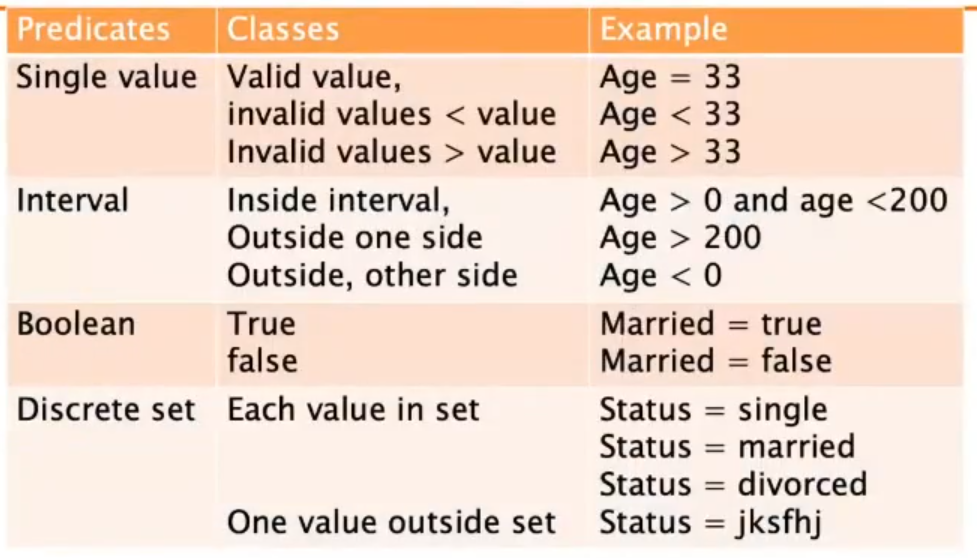
\includegraphics[width=0.8\textwidth]{equivalence-class.png}
  \caption{Equivalence Class}
  \label{fig:equivalence-class}
\end{figure}
When building black box testing we need to write a table with all the combinations of the criteria (also boundry need to be included).



In javascript it's possible to create a test by writing
\begin{lstlisting}[language=js]
import app from 'app';

describe('test suite 1', () => {
  test('T1: convert "123" -> 123', async() => {
    const res = app.convert('123');
    expect(res).toBe(123);
  });

  test('T2: convert "1d3" -> error', async() => {
    expect(() => app.convert('1d3')).toThrow(Error);
  });
});
\end{lstlisting}



\subsection{Lab}
\subsubsection{Exercise 1}
\begin{lstlisting}[language=]
boolean acceptableToEat(int carb, int protein, int fat);

The function acceptableToEat receives the weight in grams of, respectively, carbohydrates, proteins, fats in a serving of food. It returns true if
- the total amount of calories is < 1000
- (carb + protein) / fat > 1/2
\end{lstlisting}
\textbf{Criteria}:
\begin{center}
  \begin{tabular}{|l|l|}
    \hline
    Criterion Id & description \\
    \hline
    C1: totCalories & total calories \\
    \hline
    C2: fat & fat input \\
    \hline
  \end{tabular}
\end{center}
\textbf{Predicates}:
\begin{center}
  \begin{tabular}{|l|l|}
    \hline
    CId & Predicate \\
    \hline
    totCalories & 1/2 $<$ totCalories $<$ 1000 \\
    \hline
    & 0 $<$ totCalories $<$ 1/2 \\
    \hline
    & totCalories $>$ 1000 \\
    \hline
    fat & fat $>$ 0 \\ 
    \hline
  \end{tabular}
\end{center}
\textbf{Boundaries:}
\begin{center}
  \begin{tabular}{|l|l|}
    \hline
    Criterion & Boundary \\
    \hline
    totCalories & totCalories == 1/2 \\
    \hline
    & totCalories == 0 \\
    \hline
    & totCalories == 1000 \\
    \hline
    fat & fat == 0 \\
    \hline
  \end{tabular}
\end{center}
\textbf{Equivalence classes and tests:}
\begin{center}
  \begin{tabular}{|l|l|l|l|}
    \hline
    totCalories & fat & Valid & Test case \\
    \hline
    any & == 0 & n & \texttt{T1(any, any, 0):error} \\
    \hline
    (0, 1/2] & (0, inf) & y & \texttt{T2(1/3):false} \\  
     & & & \texttt{T3B(1/2):false} \\
    \hline
    (1/2, 1000) & (0, inf) & y & \texttt{T4(10):true} \\
    \hline
    [1000, inf) & (0, inf) & y & \texttt{T5B(1000):false} \\
     & & & \texttt{T6(1010):false} \\
    \hline
  \end{tabular}
\end{center}


\subsubsection{Exercise 2}
\begin{lstlisting}[language=]
double computeFee (int duration, int minRate, int minRate2);

This function computes (in euros) the fee for a bicycle rental, using these parameters
    * duration: minutes the bicycle has been used
    * minRate: cost per minute, in cents of euro
    * minRate2: cost per minute, in cents of euro
The fee is computed as follows: free the first 30 minutes. minRate per min for the first hour exceeding the first 30 min (30 to 90 minutes), minRate2 after 90 minutes
\end{lstlisting}
\textbf{Criteria}:
\begin{center}
  \begin{tabular}{|l|l|}
    \hline
    Criterion Id & description \\
    \hline
    duration & bicycle rental minutes \\
    \hline
  \end{tabular}
\end{center}
\textbf{Predicates}:
\begin{center}
  \begin{tabular}{|l|l|}
    \hline
    CId & Predicate \\
    \hline
    duration & 0 $<$ duration $<$ 30 \\
    \hline
    & 30 $<$ duration $<$ 90 \\
    \hline
    & duration $>$ 90 \\
    \hline
  \end{tabular}
\end{center}
\textbf{Boundaries:}
\begin{center}
  \begin{tabular}{|l|l|}
    \hline
    Criterion & Boundary \\
    \hline
    duration & duration == 0 \\
    \hline
    & duration == 90 \\
    \hline
  \end{tabular}
\end{center}
\textbf{Equivalence classes and tests:}
\begin{center}
  \begin{tabular}{|l|l|l|l|}
    \hline
    duration & fee & Valid & Test case \\
    \hline
    $>$ 0 \&\& $<$ 30 & == 0 & x & T1B \\
    \hline
    $>$ 30 & $>$ 0 &  & T2B \\
    \hline
  \end{tabular}
\end{center}

\subsubsection{Exercise 3}
\begin{lstlisting}[language=]
double computeFee(double basePrice, int n_passengers, int n_over18, int n_under15);

A railway company offers the possibility to people under 15 to travel free. The offer is dedicated to groups from 2 to 5 people travelling together.

For being eligible to the offer, at least a member of the group must be at least 18 years old. If this condition applies, all the under 15 members of the group travel free, and the others pay the Base Price.

The function computeFee receives as parameters basePrice (the price of the ticket), n_passengers (the number of passengers of the group), n_over18 (the number of passengers at least 18 old), n_under15 (the number of passengers under 15 years old). It gives as output the amount that the whole group has to spend. It gives an error if groups are composed of more than 5 persons.
\end{lstlisting}
\textbf{Criteria}:
\begin{center}
  \begin{tabular}{|l|l|}
    \hline
    Criterion Id & description \\
    \hline
    C1 & basePrice \\
    \hline
    C2 & npassengers \\
    \hline
    C3 & over18 \\
    \hline
    C4 & under18 \\
    \hline
  \end{tabular}
\end{center}
\textbf{Predicates}:
\begin{center}
  \begin{tabular}{|l|l|}
    \hline
    CId & Predicate \\
    \hline
    C1 & basePrice $>$ 0 \\
    \hline
    C2 & 2 $<$ npassengers $<$ 5 \\
    \hline
    & 0 $<$ npassengers $<$ 2 \\
    \hline
    & npassengers $>$ 5 \\
    \hline
    C3 & over18 $>$ 0 \\
    \hline
    C4 & under18 $>$ 0 \\
    \hline
  \end{tabular}
\end{center}
\textbf{Boundaries:}
\begin{center}
  \begin{tabular}{|l|l|}
    \hline
    Criterion & Boundary \\
    \hline
    basePrice & basePrice == 0 \\
    \hline
    npassengers & npassengers == 2 \\
    \hline
    over18 & over18 == 0 \\
    \hline
    under18 & under18 == 0 \\
    \hline
  \end{tabular}
\end{center}
\textbf{Equivalence classes and tests:}
\begin{center}
  \begin{tabular}{|l|l|l|l|l|l|}
    \hline
    basePrice & npassengers & over18 & under18 & Valid & Test case \\
    \hline
     & $>$ 5 & & & & T1 \\
     \hline
     $>$ 0 & $>$ 0 & $>$ 0 & $>$ 0 & x & T2B \\
    \hline
     $>$ 0 & $>$ 0 & == 0 & $>$ 0 & x & T3 \\
    \hline
  \end{tabular}
\end{center}







\newpage
\section{Requirement Engineering}
The aim of requirement engineering is to define the \emph{properties of the product} before starting implementation. When defining the functionality there is one or more non-functional property associated. Requirement engineering is divided into:
\begin{itemize}
  \item \textbf{Elicitation}: talk to the end-user and understand what they want
  \item \textbf{Analysis and formalization}: writing down the 
  \item \textbf{Inspection}: checking what it has been written down on the documents
\end{itemize}
\begin{definition}{Stakeholder}{stakeholder}
  In elicitation the person in charge of the requirements has to extract all information to create the requirements, the stakeholder is the \emph{person or company} that is involved in the building of the project. The stakeholder may be: user, administrator, buyer, analyst, developer.
\end{definition}
The starting point is an informal description of the problem, usually they contain defects like: omission, inconsistencies, ambiguity. The best document is the most concise one and doesn't contain omissions, this is called \textbf{complete and consistent}.
\begin{example}{Stackeholder}{stackeholder}
  \begin{itemize}
    \item POS in a supermarket.
    \item User:
      \begin{itemize}
        \item cashier at POS (profile 1)
        \item administrator, inspector (profile 2)
        \item customer at POS
      \end{itemize}
    \item Administrator:
      \begin{itemize}
        \item POS application administrator (profile 3)
        \item IT administrator (profile 4)
        \item ...
      \end{itemize}
    \item Buyer:
      \begin{itemize}
        \item CEO of supermarket
      \end{itemize}
  \end{itemize}
\end{example}



\subsection{Context Diagram}
The context diagram tells what is the focus of the requirements. The context diagram contains the \textbf{actors} of the system which can interact with it, the system is called \textbf{use case} and there can be more than one. The context diagram defines the \textbf{interface} between the inside and outside.


\begin{example}{EZGas}{ezgas}
  \emph{"EZGas is an application to help drivers find gas at lowest prices. Gas station owners can register their gas station with prices and eventually discounts. Users look for gas stations closest to them and with best prices and quality of service."}
  
  \hfill

  \textbf{1. Stakeholder}
  \textbf{Users}: 
  \begin{itemize}
    \item Person looking for a gas station;
    \item Owner of the gas station;
    \item Workers of the gas station;
  \end{itemize}
  \textbf{Administrator}:
  \begin{itemize}
    \item App database(s) administrator;
    \item Local gas station administrator;
    \item Money transaction administrator;
  \end{itemize}
  \textbf{Buyers}: 
  \begin{itemize}
    \item Local gas station owners;
  \end{itemize}
  \textbf{2. Context diagram and interface}
  \begin{figure}[H]
    \centering
    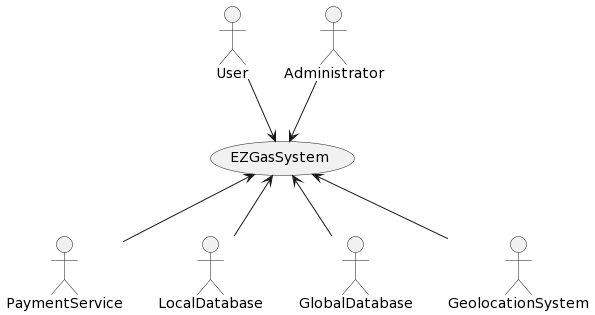
\includegraphics[width=0.8\textwidth]{context-diagram-ezgas.png}
    \caption{Context Diagram EZGas}
    \label{fig:context-diagram-ezgas}
  \end{figure}
  \begin{table}[H]
    \centering
    \begin{tabular}{|c|c|c|}
      \hline
      \textbf{Actor} & \textbf{Physical Interface} & \textbf{Logical Interface} \\
      \hline
      User & Smartphone, Internet & GUI \\
      \hline
      Administrator & Screen, Keyboard & GUI, shell \\
      \hline
      Payment System & Internet & API \\
      \hline
      Geolocation System & Internet & API \\
      \hline
      Local/Global Database & Keyboard, Internet & shell, API \\
      \hline
    \end{tabular}
    \caption{Interface Table}
  \end{table}
  \textbf{3. Functional Requirements}
  \begin{table}[H]
    \centering
    \begin{tabular}{|l|l|}
      \hline
      f1 & user authentication \\
      \hline
      f1.1 & use authentication token \\
      \hline
      f1.2 & register unregistered users \\
      \hline
      f1.3 & create new account \\
      \hline
      f2 & search gas station \\
      \hline
      f2.1 & choose search options \\
      \hline
      f2.1.1 & closest gas station \\
      \hline
      f2.1.2 & best price gas station \\
      \hline
      f2.1.3 & closest/best price mix gas station \\
      \hline
      f2.2 & select fuel kind \\
      \hline
      f2.3 & select most green company \\
      \hline
      f3 & user becoming gas station owner \\
      \hline
      f3.1 & add owned gas station \\
      \hline
      f3.1.1 & add discount \\
      \hline
      f3.1.2 & remove discount \\
      \hline
      f3.1.3 & modify gas prices \\
      \hline
      f3.1.4 & modify gas kinds \\
      \hline
      f3.2 & pay periodical fee \\
      \hline
    \end{tabular}
  \end{table}
  \textbf{5. Table of rights}
  \begin{table}[H]
    \centering
    \begin{tabular}{|l|l|l|}
      \hline
      \textbf{Actor} & \textbf{User} & \textbf{Owner} \\
      \hline
      f1 & \checkmark & \checkmark \\
      \hline
      f2 & \checkmark & \checkmark \\
      \hline
      f3 &  & \checkmark \\
      \hline
    \end{tabular}
  \end{table}
\end{example}

\hfill

\begin{example}{Robotic Vaccum Cleaner}{robotic-vaccum-cleaner}
  \emph{"Since several years robotic vacuum cleaners (RVC) are available. An RVC is capable of cleaning the floors of a house in autonomous mode. An RVC system is composed of the robot itself and a charging station. The charging station is connected to an electric socket in the house, and allows charging the battery on board of the robot. The robot itself is composed of mechanical and electric parts, a computer, and sensors. One infrared sensor in the frontal part recognizes obstacles, another infrared sensor always on the frontal part recognizes gaps (like a downhill staircase). A sensor on the battery reads the charge of the battery. The computer collects data from the sensors and controls the movement of four wheels. Another sensor on one of the wheels computes direction and distance travelled by the robot. Finally, on top of the robot there are three switches: on-off, start, learn. The learn button starts a procedure that allows the robot to map the space in the house. With a certain algorithm the robot moves in all directions, until it finds obstacles or gaps, and builds an internal map of this space. By definition the robot cannot move beyond obstacles, like walls or closed doors, and beyond gaps taller than 1 cm.  The starting point of the learn procedure must be the charging station. When the map is built the robot returns to the charging station and stops.  The start button starts a cleaning procedure. The robot, starting from the charging station, covers and cleans all the space in the house, as mapped in the ‘learn’ procedure. In all cases when the charge of the battery is below a certain threshold, the robot returns to the charging station. When recharged, the robot completes the mission, then returns to the charging station and stops."}

  \hfill
  
  \textbf{Business Model:}
  \begin{itemize}
    \item Private Company;
    \item Customers buy the RVC;
    \item Customers can bring RVC to assistance;
    \item Expert Customers can buy spare parts;
  \end{itemize}
  \textbf{1. Stakeholders:}
  \begin{itemize}
    \item Users:
      \begin{itemize}
        \item Customers;
        \item Technicians;
      \end{itemize}
    \item Administrators:
      \begin{itemize}
        \item Firmware administrator;
        \item Components administrator;
      \end{itemize}
    \item \textbf{Buyers:}
      \begin{itemize}
        \item Customer;
        \item Components Companies;
      \end{itemize}
  \end{itemize}
  \textbf{2. Context Diagram:}
  \begin{figure}[H]
    \centering
    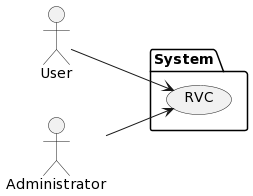
\includegraphics[width=0.3\textwidth]{rvc-context-diagram.png}
    \caption{RVC Context Diagram}
    \label{fig:rvc-context-diagram}
  \end{figure}
  \begin{table}[H]
    \centering
    \begin{tabular}{|c|c|c|}
      \hline
      \textbf{Actor} & \textbf{Physical Interface} & \textbf{Logical Interface} \\
      \hline
      Customer & Buttons & - \\
      \hline
      Administrator & Keyboard & USB \\
      \hline
    \end{tabular}
  \end{table}
  \textbf{3. Functional Properties:}
  \begin{table}[H]
    \centering
    \begin{tabular}{|l|l|}
      \hline
      f1 & perform action \\
      \hline
      f1.1 & start/stop learning \\
      \hline
      f1.2 & start/stop cleaning \\
      \hline
      f1.3 & start/stop charging \\
      \hline
      f1.4 & return to charging station \\
      \hline
      f1.5 & return to previous action \\
      \hline
      f2 & firmware update \\
      \hline
      f3 & factory reset \\
      \hline
      f4 & read data from sensors \\
      \hline
    \end{tabular}
  \end{table}
  \textbf{5. Table of Rights}
\end{example}



\section{UML}
Thanks to UML (\emph{Unified Modeling Language}) it's possible to represent the relationships between the various objects of the system. UML has many characteristics, some of which are (it the case of \emph{UML Class Diagrams}):
\begin{itemize}
  \item The Object is the \textbf{Model} of an item, every Object \emph{has unique ID}.
  \item \textbf{Class} is the descriptor of a set of items that can be grouped together.
  \item Classes can be \textbf{associated}.
  \item Every Class has \textbf{Attributes}.
\end{itemize}
In UML different class can be \emph{linked} together, this is called \textbf{Association} and represent a logical relationship between them, the association can unidirectional or bidirectional, also classes may have more than one link to represent different logical concepts. When links are formed between classes there can multiplicity of the number of classes dependent:
\begin{itemize}
  \item \texttt{1}
  \item \texttt{0..1}
  \item \texttt{0..n}
  \item \texttt{1..n}
  \item \texttt{m..n}
\end{itemize}
The \textbf{role} is how what a class represent when it has an association. This comes useful when \textbf{recursive associations} are present.

\hfill

\textbf{Composition} is indicated with a \emph{diamond}, it represent when a Class is a \emph{component} of another one, this takes a different approach with respect to inheritance, and there are two kinds:
\begin{itemize}
  \item When the diamond \textbf{is hollow} and \emph{the class A which points to B} means that, \emph{A} is part of \emph{B}.
  \item When the diamond \textbf{is full} the lifecycle are all associated, if a component dies all the other component die too.
\end{itemize}
\textbf{Generalization} is a way to implement inheritance, the parent class is pointed by a \emph{hollow arrow}. The parent class is a more generalized class, all the attributes of the generalized class are inherited by his children.


Before starting the project with UML it is import to define what are his context, e.g.:
\begin{itemize}
  \item model of concepts (glossary);
  \item model of system (system design);
  \item model of software classes;
  \item model of deployment (deployment diagram);
\end{itemize}
\emph{It's always important to minimize the number of classes.}




\subsection{Glossary}
The \textbf{glossary} or \textbf{conceptual diagram} is a way to describe the objects of our system processing. Thanks to \emph{UML Class Diagram} it's possible to represent the relationships between the various objects of the system. The glossary it's different from the \textbf{System Design}, in fact during this phase the design of the various software component must not be considered, for example the glossary representation of a university is the following:
\begin{figure}[H]
  \centering
  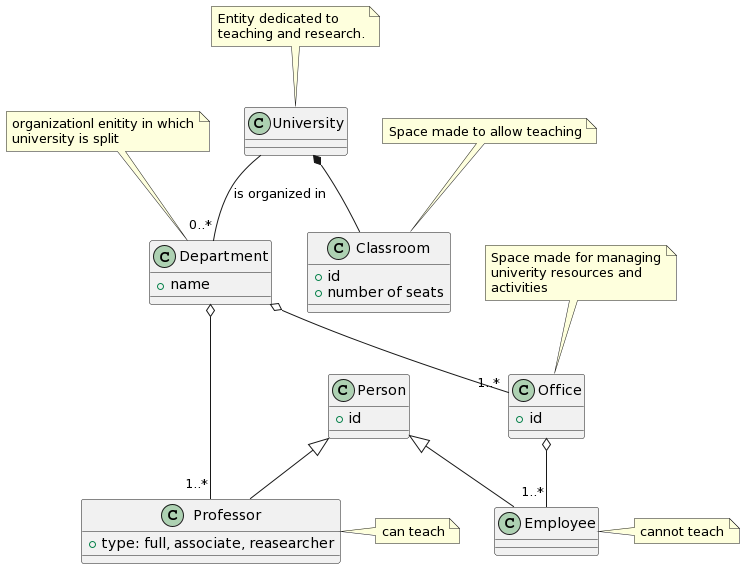
\includegraphics[width=0.8\textwidth]{university-uml-diagram.png}
  \caption{University UML Diagram}
  \label{fig:university-uml-diagram}
\end{figure}
If the name of the class is not self-explanatory a note is recommended to explain what that is or does.


\subsection{System Design}
On the other hand a \textbf{System Design} shows how the software parts of the system are related to one another, the system design can have different granularity, ranging from the representation of an entire software app reduced to a Class, to represent the real software Classes inside the application.

\subsection{UML Deployment Diagram}
The \textbf{deployment diagram} is a way to represent how the system is deployed on the physical hardware, and it uses \emph{UML Deployment Diagram}, in general every physical device is represented with a \textbf{node}, and the piece of software, library, or file that is \emph{deployed} on that physical device is called \textbf{artifact}.
\begin{figure}[H]
  \centering
  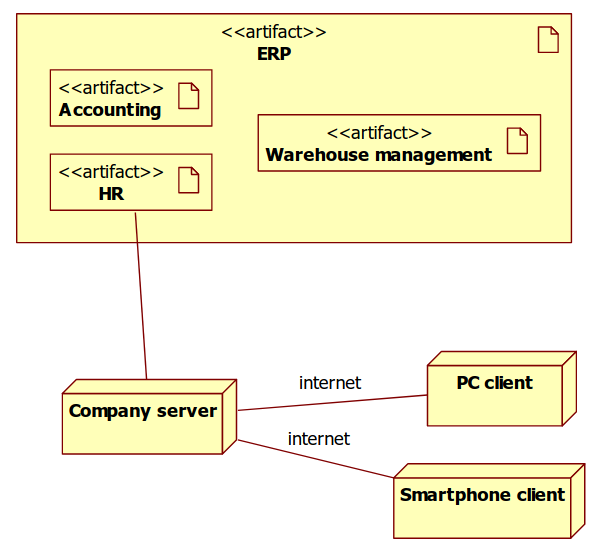
\includegraphics[width=0.6\textwidth]{deplyment-diagram-example.png}
  \caption{Deployment Diagram Example}
  \label{fig:deplyment-diagram-example}
\end{figure}

\begin{example}{Lab2 EZGas}{lab2}
  \textbf{6. Glossary}
  \begin{figure}[H]
    \centering
    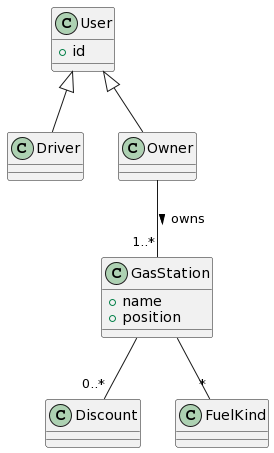
\includegraphics[width=0.4\textwidth]{ezgas-glossary.png}
    \caption{Ezgas Glossary}
    \label{fig:ezgas-glossary}
  \end{figure}
  \textbf{7. System Design}
  \begin{figure}[H]
    \centering
    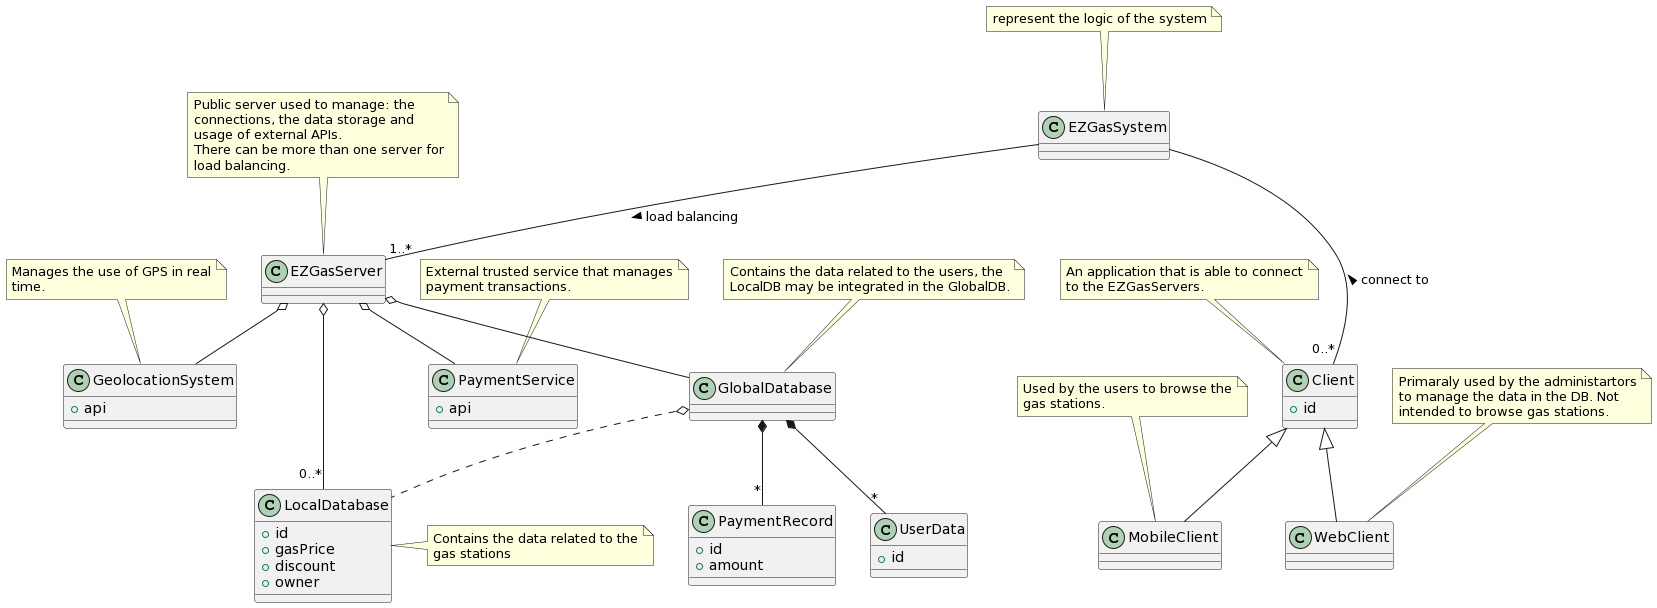
\includegraphics[width=1\textwidth]{ezgas-system-design.png}
    \caption{Ezgas System Design}
    \label{fig:ezgas-system-design}
  \end{figure}
  \textbf{8. Deployment Diagram}
  \begin{figure}[H]
    \centering
    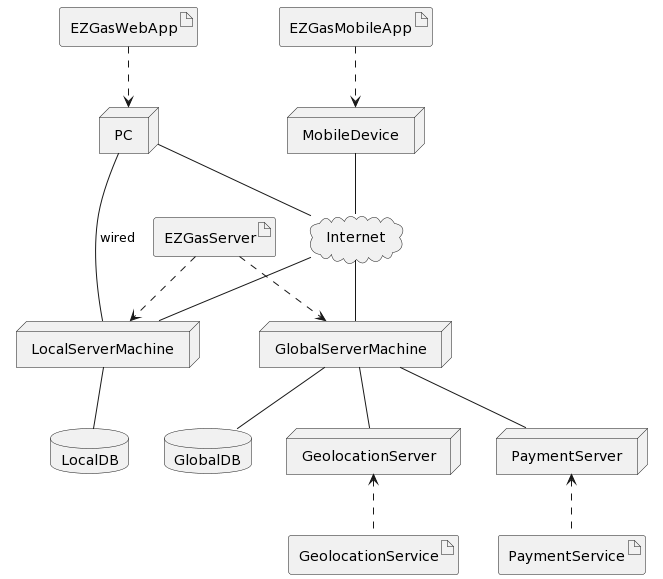
\includegraphics[width=0.8\textwidth]{ezgas-deployment-diagram.png}
    \caption{Ezgas Deployment Diagram}
    \label{fig:ezgas-deployment-diagram}
  \end{figure}
\end{example}

\hfill

\begin{example}{Lab2 RVC}{lab2-rvc}
  \textbf{6. Glossary}
  \begin{figure}[H]
    \centering
    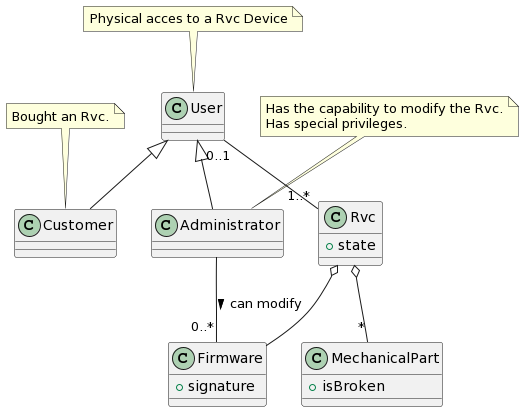
\includegraphics[width=0.6\textwidth]{rvc-glossary.png}
    \caption{Rvc Glossary}
    \label{fig:rvc-glossary}
  \end{figure}
  \textbf{7. System Diagram}
  \begin{figure}[H]
    \centering
    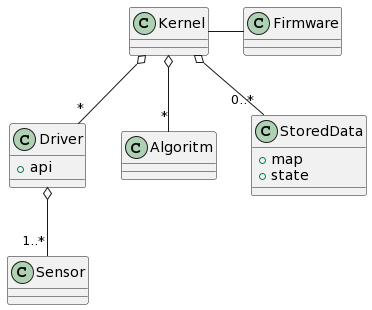
\includegraphics[width=0.4\textwidth]{rvc-system-design.png}
    \caption{Rvc System Design}
    \label{fig:rvc-system-design}
  \end{figure}
  \textbf{8. Deployment Diagram}
  \begin{figure}[H]
    \centering
    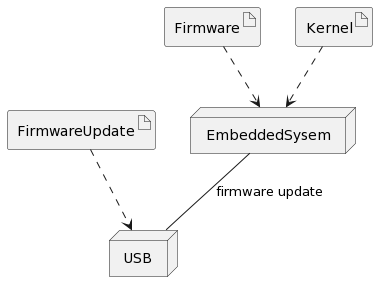
\includegraphics[width=0.4\textwidth]{rvc-deployment-diagram.png}
    \caption{Rvc Deployment Diagram}
    \label{fig:rvc-deployment-diagram}
  \end{figure}
\end{example}


\subsection{Use Cases and Scenarios}
A \textbf{scenario} is a story. To build a scenario we start from the \textbf{context diagram}, and the focus of the scenario is about explaining how the actors interact with the interfaces. Every scenario described is described with steps about what is going to happen.

On the other hand the \textbf{usecase} is the visual description of how the actor are related to the functional requirements of the system and the steps that they have to take.





\section{Non-Functional Requirements}
Non-functional requirements are some kind of properties associated to a functional property. There are some defined standard non-functional properties which are: usability, efficiency,

\textbf{Usability}: usability could be measured in:
\begin{itemize}
  \item effort to learn: to do this is experiment we can take a number of users (non-technical) and observe their responses;
\end{itemize}

\textbf{Efficiency}: represent the response time and the resource used (usually computed for the whole application, it's difficult to calculate the efficiency for a single functionality).

\textbf{Correctness}: capability of writing the right functionality, this is always unfeasible.


\textbf{Reliability}: it is the probability to encounter a defect over a period of time, the defects are bugs visible to the end-user.

\textbf{Maintainability}: is the maximum effort to operate a change on the software.

\textbf{Portability}:

\textbf{Security}: protection from malicious attacks.

\textbf{Safety}: the system is safe if it cannot harm any person or get into a hazardous situation, if it does so it needs to have some kind of control.

\textbf{Dependability}:

\subsection{EZGas}
\textbf{Scenarios and Usecases}
\begin{itemize}
\begin{figure}[H]
  \centering
  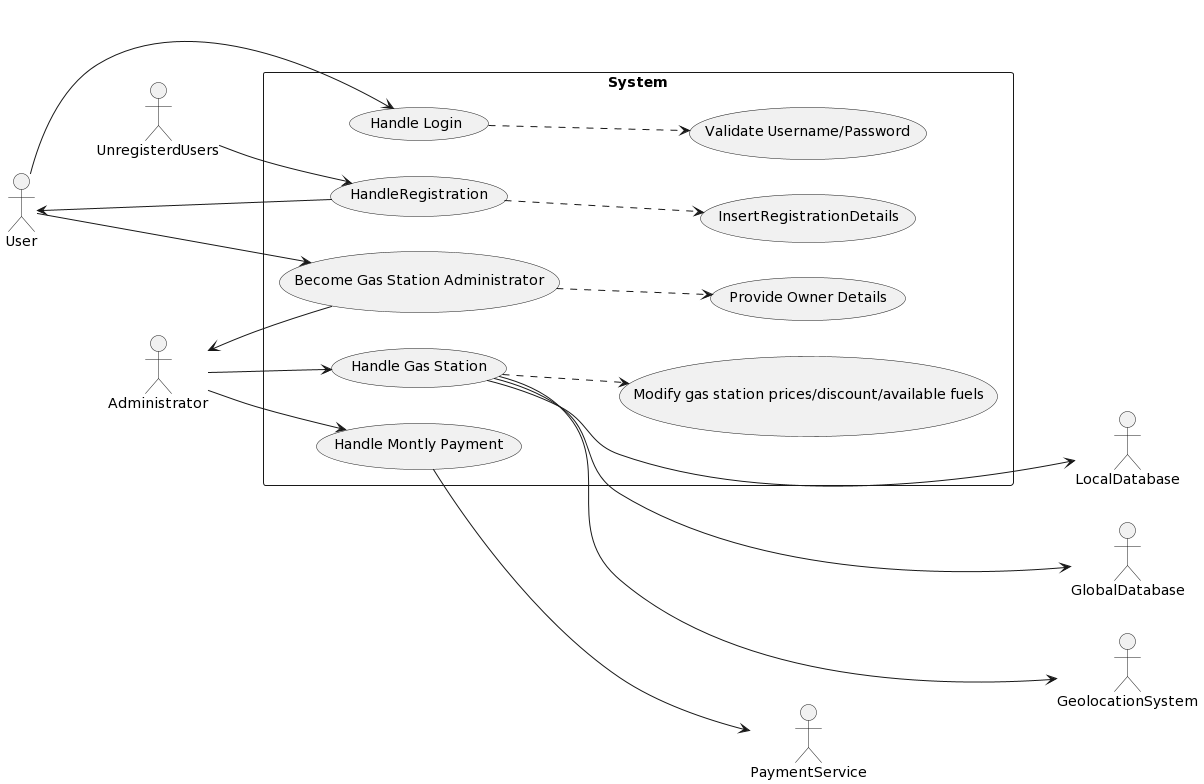
\includegraphics[width=1\textwidth]{ezgas-usecase-diagram.png}
  \caption{Ezgas Usecase Diagram, \href{http://www.plantuml.com/plantuml/uml/PP31Rjim38RlVWgXzpGlC1JTKA0Ri6B1WkvEMun3G9O2ad9X37ltIQnS9-WXWSdl9_NpVnG5rZo5Bk19dIR7D9xLUM8Sb5BiEXWqiNkDZ2E98ljNGHO7ud9ki7QiqUglVg9On0oQ3403pvX26g0kFYwYE5KuIgC7M2QCUaIUQS2ABYlwMQR24oZq84Q2xzUT8VMtR2oiw-e14CU0hZtrj-kou515to7wWB_j8ZOxTUxC7u8VKP3rMl242XJiRcA_hRfxtrKSZXJlAhQlZV-1G1uKBQK84-uF8FAMs9jwRlXgupSSqeJkkT2ZskEtYThS26BDRUp0QIQFxjTRH7RDhscJH_ti-2L53SkQkWali7pINVim4KNPD2_9qscfRfmqhnUc0MNlIOQKe-vX1WhGbqsdZCtHb4g4_yfRsUrs3pNvCxlx-mVBDhilkrtj5LvnIzJ-JRHcPhm8jZ3QXydQsM3RLb1gMscNbh_tGbhRRYi_6pUFjR0dWk-tOhmff7l4wFCK_WC0}{Link} }
  \label{fig:ezgas-usecase-diagram}
\end{figure}
  \item \textbf{UC: Login}
    \begin{itemize}
      \item Precondition:
        \begin{itemize}
          \item User is not authenticated and not authorized;
          \item User must be registerd;
        \end{itemize}
      \item Postcondition:
        \begin{itemize}
          \item User is authenticated and authorized;
        \end{itemize}
    \end{itemize}
    \begin{enumerate}
      \item User enters the app;
      \item Inserts username and passwords;
      \item Repeat until username and passwords are correct;
      \item User is logged in;
    \end{enumerate}
  \item \textbf{UC: Registration}
    \begin{itemize}
      \item Precondition:
        \begin{itemize}
          \item Download the app;
        \end{itemize}
      \item Postcondition:
        \begin{itemize}
          \item User has an account associated to a username and password;
        \end{itemize}
    \end{itemize}
    \begin{enumerate}
      \item User enters the app;
      \item Click the sign in button;
      \item Isert his username;
      \item Repeat until a valid username;
      \item Insert password;
      \item Repeat until a valid password;
      \item Insert email for password recovery;
      \item Verify email;
      \item User is now registrated;
    \end{enumerate}
  \item \textbf{User Needs Gas Station}
    \begin{itemize}
      \item Precondition: user logged in;
      \item Postcondition: user finds gas station;
    \end{itemize}
    \begin{enumerate}
      \item Users may set custom parameter for searching a gas station;
      \item User is prompted with a gas station;
      \item User may decline the gas station, if declined repeat previus step;
      \item User drives to gas station following the map instructions;
      \item User arrives;
      \item User completes his journey;
    \end{enumerate}
  \item \textbf{User Becomes GasStation Administrator}
    \begin{itemize}
      \item Precondition: user is logged in;
      \item Postcondition: user is now a gas station administrator;
    \end{itemize}
    \begin{enumerate}
      \item User wants to become a gas station owner;
      \item User enrolls to become a gas station owner;
      \item User provides his details: partita IVA;
      \item User pays monthly fee;
      \item User becomes Administrator;
    \end{enumerate}
  \item \textbf{Administrator Add GasStaion}
    \begin{itemize}
      \item Precondition: user is an administrator, administartor has acces to local/global db;
      \item Postcondition: a new gas station is added the EZGas system;
    \end{itemize}
    \begin{enumerate}
      \item Admin enters gas station owner area in the application;
      \item Admin can add or remove his owned gas stations;
      \item Admin adds all the kinds of fuel present in a gas station;
      \item Admin can add or remove discounts present for a fuel in a gas station;
      \item Changes are submitted;
      \item Validation is received from the server;
    \end{enumerate}
\end{itemize}
\textbf{Non-Functional Requirements}
\begin{itemize}
  \item The app shall be developer for iOS, Android, Web;
  \item Avarage users should be able to learn how to use the basic functionality of the app in 10 minutes
  \item The application must satisfy the requirements of GDPR (EU) and CCPA (California) for the satisfaction of the app security.
  \item A time of 20 hour person (5 persons in a week development) to add a new feature.
  \item To develop an app for iOS, Android, Web shall take 6 months for the initial deplyment.
  \item The map must be updated once a week to avoid bringing the users into hazardous situations like: work in progress zone, accident site, ...
  \item The application server needs to have an \emph{up-time} of $99\%$ during the span of a year.
  \item The application 
\end{itemize}





\newpage
\section{User Interface}
Typcally the user interface represent a human interacting with the graphical interface of the program. Usually when we start to build a UI for our applications we need to start from: \textbf{context diagrams and actors}, \textbf{function requirements} and esecially \textbf{use cases}. When looking at our use cases we can the steps that an actor is performing and the UI should represent this steps in simple way. A key idea to always remember is to \emph{keep the UI simple}, in fact \emph{"A user interface is like a joke. If you have to explain it, it's not that good"}, also another key aspect of implementing a UI is \textbf{experimentation}.

The context is also important, in fact nowadays the applications can be developed for many differet devices, like: desktop, web, mobile phone, smartwatch, etc...

As a principle we should use the \textbf{simpicity}, we can represent it with three different axes, which are all related to each other, and we should remain as close to the orgin as possible.
\begin{figure}[H]
  \centering
  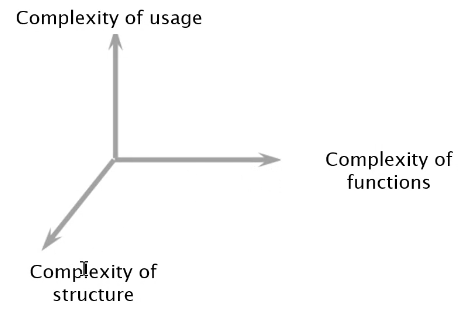
\includegraphics[width=0.4\textwidth]{ui-simplicity.png}
  \caption{Ui Simplicity}
  \label{fig:ui-simplicity}
\end{figure}
Obviously the simplicity of the interface depends on the funcionality that it is built on, if for example we are building an application to pilot a shuttle to the ISS, it's not a very good idea to implent the controller with three buttons, obviosly shuch application will have thousends of lines of code and hundreds of buttons to control every funcitonality, that's way the context of build a UI is very important.

\hfill

The main approaches for designing an interface are:
\begin{itemize}
  \item \textbf{Ergonomy}: safety, adaptability, comfort, usability, one entry point, ...
  \item \textbf{Emotional Design}: is about the emotion about using a certain device raise in a user using it, like Apple products.
  \item \textbf{User Experience (UX)}: usability + feelings + emotions + values.
\end{itemize}
We also need to keep in mind the at the end of day the end-user will interact with the UI and so our choices needs to based on \emph{feedback from the real user}, and not on our personal opinion, this is called \textbf{User Centered Design (UCD)}. The UCD has five steps:
\begin{figure}[H]
  \centering
  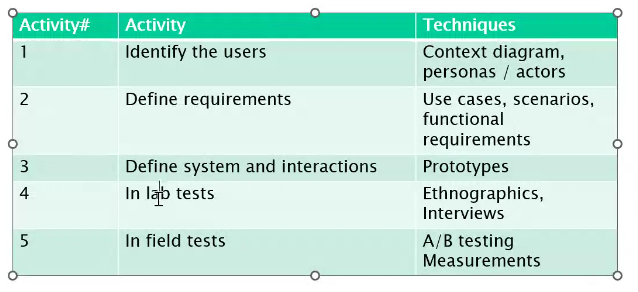
\includegraphics[width=0.8\textwidth]{user-centered-design-process.png}
  \caption{User Centered Design Process}
  \label{fig:user-centered-design-process}
\end{figure}



\subsection{Prototype}
A proptotype is a simplified version of the final version of the interface. The inital steps can be made on: paper, postit, sketches, ... (\textbf{Low Fidelity}: needs to be done fast). The next step is by producing \textbf{High Fidelity} UI, this is done by using a computer, there are many products to do this, like: \textbf{Balsamiq}, \textbf{Figma}, ... The final step will be to use an \emph{actual GUI Builder}, which will generate all the software calsses and all the methods needed to link the software and his functionality with the GUI.


\subsection{In Lab Tests}
The test are done via interviews with the users or in a monitored environment.


\subsection{In Field Tests}

For example a way to get feedback from a deplyed system is the A/B test.
\begin{figure}[H]
  \centering
  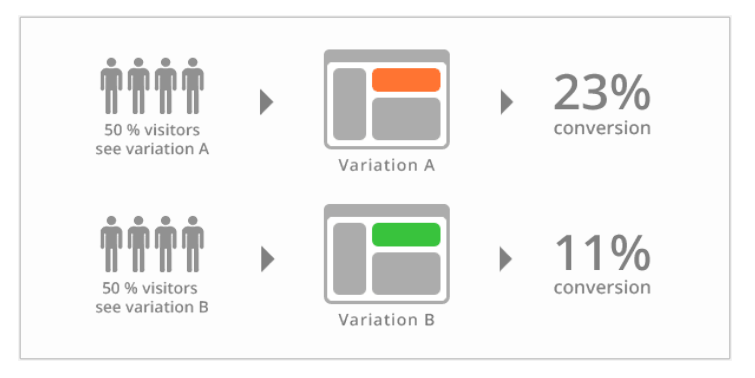
\includegraphics[width=0.8\textwidth]{a-b-test.png}
  \caption{A B Test}
  \label{fig:a-b-test}
\end{figure}
This is typacally done: the users are split in two sets which there is a functionality has a variation injected to the two subsets, if the feature has a far greater use in a scenario then that will be the final choice on the application.


\subsection{GUI Design}

Usability Guidelines ......

After many years there are some conventions used in the design of a product: 
\begin{itemize}
  \item logo at top left;
  \item click on logo brings home;
  \item links change color on mouse hover;
  \item next/back is always in the same place;
\end{itemize}



\newpage
\section{Project Mangement}
Before starting a project there are the Estimantion document which contains the the estimations for when the project will be ready and how much time the project will require, this is what project managemtn tries to answer to.

The planning of the project and the cantract between company and buyer are called \textbf{Inception Phase}, this phase is payed by the company which is producing the estimation documents, only if the buyer will accept all the terms then there will somt profit, otherwise the company operates at a loss.

During the \textbf{Development Phase}, it's important to keep track of the time and resources pent on the project.

\begin{itemize}
  \item \textbf{Project}: collaborative endeavour to achieve  a goal, wiht define limits of time/money;
  \item \textbf{Program}: managemtn of several related projects (e.g. \emph{Apollo Program});
\end{itemize}
A project can be:
\begin{itemize}
  \item \textbf{bespoke}: e.g. polito app;
  \item \textbf{commercial}: e.g. MS Windows;
\end{itemize}

\subsection{Measures}
Some of the measurament variants are: estimated value, actual value, targe value (what is desirable), benchmark (what the others do).

Project is basically a way to keep toghter: calendar time, cost, functionality and quality.

The first measure is \textbf{Duration}, which is dived in absolute and relative, eventually relative will be transalted into absoute.

\textbf{Effort} is defined as $p * h$, where $p$ is the number of persons and $h$ is the number of hours. 
What is the realtion between cost and price? The siplest model is: price = cost + margin.

TCO: ...

The \textbf{Size} of a sofware product is usually defined as Lines of Code (LOC) even though it's not very precise.




\subsection{Techiques}
\textbf{WBS} Work Breakdown Structure: you have a certain activity, and then this is divied in smaller activities (divide and conquer), in WBS there is no temporale relationshipt.

\textbf{Gantt Chart}
\begin{figure}[H]
  \centering
  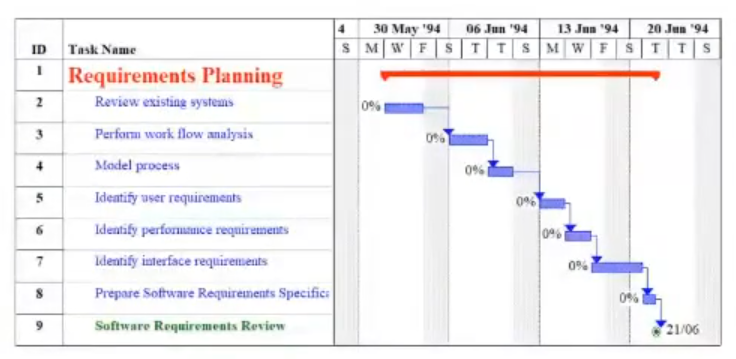
\includegraphics[width=0.8\textwidth]{gantt-chart.png}
  \caption{Gantt Chart}
  \label{fig:gantt-chart}
\end{figure}
On the left there are the various the WBS, on the right each bar is calendar time of each WBS, and they are put with temporal relationship.

The \textbf{PBS (Product Breakdown Structure)}, is the heirarchical structure of a project.

The planning process aims to:
\begin{itemize}
  \item estimate the effort and cost;
  \item identify acitivities: PBS, WBS
  \item define schedule: Gantt
\end{itemize}



\subsection{Estimation}
Estimating a project is more easyer with more experience.

Other ways (more objective) to estimate a prject are the following techniques: 
\begin{itemize}
  \item \textbf{By decomposition}: based on WBS or PDS, then the various parts are summed up to get the totale effort;
\end{itemize}



\subsection{Tracking}
How to keep track of the project? The first step is to collect data, to do that we need to collect 


\subsection{Staffing Profile}
Typically, by increasing the number of people working on a single feature it increaces productivity up to a certain point, and then it starts to decrease, this shape follows a Bell's Curve.


\subsection{Stories and personas}
(Mettere in Requirements)

How to define how the people using our app will behave? One solutoion is using personas, this comes from the technique of fragmentation. For example people can bertitioned by:
\begin{itemize}
  \item \textbf{Domographic:} age, gender, income, religion, level of education, ...
\end{itemize}
A persona idintifies and describes typical users, and we target the application to a subset of personas, obviously it's not possible to define every subset of people.

\subsection{Elicitation}
(Da finire: Requiremnt)
We take a group of people wich coul represent the personas.
\subsubsection{Interview}
Interview people with a set of prepared questions

\subsubsection{Ethnographics}
The data collecotr is not present in the room and the people aare alone in the room, and the collector observers how to peaple behave with the app, this is also done online with tracking tool that observer how we intercat with the applications.


\subsection{Exercise}
\textbf{Exercise 1:}
...

\textbf{Exercise 2:}
A new software project has an estimated size of 210000 lines of code. Past similar projects in the same company had a productivity 30 person day.
\begin{enumerate}
  \item Esimate the effort for the new project: ouput / effort = LOC / effort
    210000 loc / 30 loc/pd = 7000 person day \\
    7000 / 140 = ... p month
  \item Estimate the duration of the porject, assuming to have 4 people available to work on it.

    7000 pd / 4 p =  1750 calendar days = 12.5 calendar months
  \item on avarage the cost of a person day is 150 Euros. Estimate the cost of the prject.

    150 * 7000 euro
\end{enumerate}

\textbf{Exercise 3:}
\begin{enumerate}
  \item Compute the effort (peron hours) estimated for developement, according to the article (assume a person wrokd 140 hours per calendar month):

    5 * 2 * 140 = 1400 ph
  \item Compute the cost per person hour, during developemnt:

    300000 / 1400 = 214 euros per person hour
  \item Discuss the estimates of time and cost for development.

    2 months seems very short time, cost very high
  \item Using the cost per person hour at point 2, compute the person hourse estimated fot eh maintanance phase, per year.

    200000 / 214 = 1000 ph = 7 pm
\end{enumerate}


\newpage
\section{VV, Inspection, Reading}
Whatever we produce can contain bugs and errors, this is why there is the last part wiich is the inpection of the work done, ...

Verification and Validation: checking that what we did is correct. Validation: doing the right software system valued by the stackeholders. Verification: is doing correctly the internal transformation.
\begin{figure}[H]
  \centering
  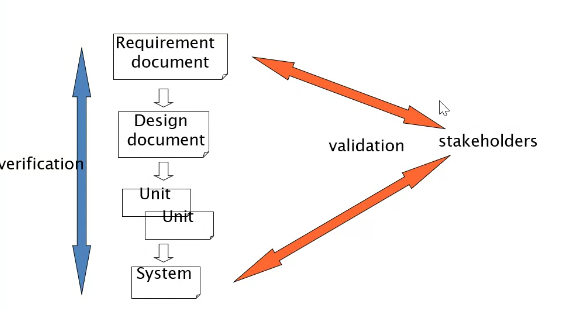
\includegraphics[width=0.8\textwidth]{vv.png}
  \caption{V\&V}
  \label{fig:vv}
\end{figure}



\subsection{Failure, Fault, Defect}
Failure is an execution event where the software behaven in unexpected way. The end-user catched the problem

Fault: a feature in software that causes a problem, error in the code or in documents.

A failure is caused by a fault. A failure may never araise, the simple reason is that that part of the code/documnents is unused.
\begin{figure}[H]
  \centering
  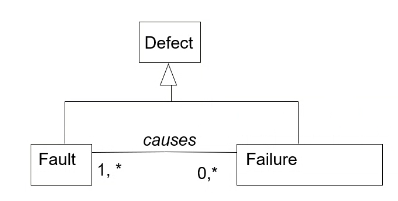
\includegraphics[width=0.8\textwidth]{failure-fault-defect.png}
  \caption{Failure Fault Defect}
  \label{fig:failure-fault-defect}
\end{figure}
Someties it's not clear what is the fault and what is the failure so can both call them defects.

\subsection{Inspections}
This is done for document checking (also applyable to code), is a reading technique and it uses group dynamic, the aim is to \textbf{find defects}.

the aim is to find the \textbf{taxonomy of the defetcs}. Find:
\begin{itemize}
  \item inconsistency
  \item abiguity
  \item ...
\end{itemize}
Another tachnique is to do a \textbf{checklist}.


\section{Architecture and Design}
Requirements: what the system shoud do; Architecture: how the system should be built. In general many differnt designs are possible, but there are some common desgin patterns. After many iterations of a disign for a product a \textbf{dominant design} will araise.

Software design is defining modules and their interactions so that they satisfy function and non-functional requiremnts (usually the most difficoult to satisfy).

Architecture: high level components are designed with their interactions, a comunication and coordination model is selected, like: process, threads; messages, procedure calls; broadcast, blackboard; so we need to select either one of them.

Design: is about high level decisions inside each component.

There are some non-functioal properties for architecture design:
\begin{itemize}
  \item testability
  \item monitorability
  \item interopelability
  \item scalability
  \item deployability
  \item mdobility
\end{itemize}
Other non-functional properties are:
\begin{itemize}
  \item complexity: minimize number of components and number of interations
\end{itemize}

Coupling: modules shoul have least amount of coupling between them, the coupling is the degree of dependance between two components.


Cohesion: we should put in the same components parts that are related to the component
\begin{itemize}
  \tolerance=1000
  \item higher: Engine: (start(), stop())
  \item lower: Engine: (start(), stop(), monitorObstacles()), monitorObstables() doesn't fit inside the Engine module, thus causing lower cohesion
\end{itemize}

...

Cost: some functionalityies are more expensive than others

Schedule: if there are more than one component they can be developed in parallel

Staff skills: the staff needs to be trained to work on a specific component.


...

Performance: minimaze number of operations and comunications, larger components

Security: use a layerd architecture, like a firewall

Safety: more control on seaty-critical features, make the subsystem

Availability: add redunt components

Maintanability: replacable components

Performance vs Security; Availability vs Security, Performance; there conficts we need a trade off, we need to choose which non-functional requirement is more important, defined by the stakeholders.

\subsection{Notations}
A simple box and line diagram, where a box is a component and an arrow is an interaction. These can also be done with UML class diagrams or packages diagrams. The sequence of function calls should never be displayed in the class diagram, to do that there is the dynamic view, that may correspond to the implementation of a use case.
\begin{wrapfigure}{L}{0.4\textwidth}
  \centering
  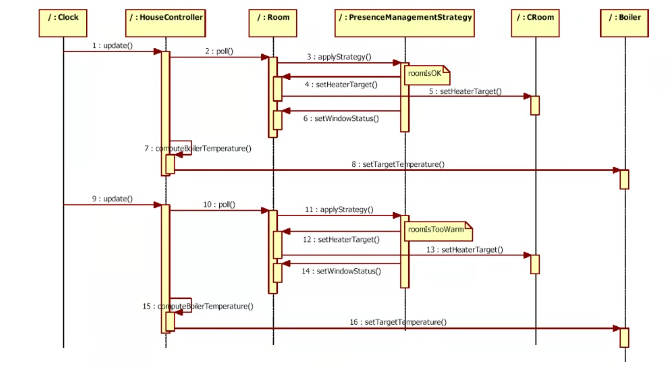
\includegraphics[width=1\linewidth]{sequence-diagram.png}
  \caption{Sequence Diagram}
  \label{fig:sequence-diagram}
\end{wrapfigure}




\subsection{Patterns}
Patterns are similar to dominant design in other engeneering fields, to solve common recurring problems. 

\subsubsection{Architecture Patterns}
\textbf{Repository style}: each interaction happens through a file system

\textbf{Client server}:

\textbf{ISO/OSI model}:

\textbf{3 tier architecture}: persentation, application login, data.

\textbf{Pipes and Filters}: like linux pipes

\textbf{MVC (Model View Controller)}: The proble with have a graphical part to display. The simplest way is to have a single class, but everithing gets messy really quickly, and having more than one representation we will have to write everithing from scratch because the logic and graphic part are tightly coupled togheter, one way of extraciting that is using a \texttt{Model} of the the grohpical part wich will contain the logic while the \texttt{View} will only contain the graphical representation, the \texttt{Controller} is what controls the flow of data on logic, for example Android uses MVC, the \texttt{Controller} is the generic \texttt{View} class, his \texttt{View} is the XML file associated, while the \texttt{Model} is the data associated with the current XML file. Usually the cycle is: \texttt{View} fire events, \texttt{Controller} update model, \texttt{Model} update view.

\textbf{Miccrokernel}: 

\textbf{Microservices}:












\end{document}

%% vim: ts=2 sts=2 sw=2 et
